\documentclass[a4paper,12pt]{ctexart} 

% First, we usually want to set the margins of our document. For this we use the package geometry.
\usepackage[top = 2.5cm, bottom = 2.5cm, left = 2.5cm, right = 2.5cm]{geometry} 
\usepackage[T1]{fontenc}
\usepackage[utf8]{inputenc}

% The following two packages - multirow and booktabs - are needed to create nice looking tables.
\usepackage{multirow} % Multirow is for tables with multiple rows within one cell.
\usepackage{booktabs} % For even nicer tables.

% As we usually want to include some plots (.pdf files) we need a package for that.
\usepackage{graphicx} 

% The default setting of LaTeX is to indent new paragraphs. This is useful for articles. But not really nice for homework problem sets. The following command sets the indent to 0.
% \usepackage{setspace}
% \setlength{\parindent}{0in}

% Package to place figures where you want them.
\usepackage{float}

% The fancyhdr package let's us create nice headers.
\usepackage{fancyhdr}

\usepackage{amsmath,amsthm,mathabx,caption,diagbox}

% To make our document nice we want a header and number the pages in the footer.

\pagestyle{fancy} % With this command we can customize the header style.

\fancyhf{} % This makes sure we do not have other information in our header or footer.

\lhead{\footnotesize Probability and Statistics: Section 3.5}% \lhead puts text in the top left corner. \footnotesize sets our font to a smaller size.

%\rhead works just like \lhead (you can also use \chead)
\rhead{\footnotesize 吴梦轩} %<---- Fill in your lastnames.

% Similar commands work for the footer (\lfoot, \cfoot and \rfoot).
% We want to put our page number in the center.
\cfoot{\footnotesize \thepage} 

\begin{document}

\thispagestyle{empty} % This command disables the header on the first page. 

\begin{tabular}{p{15.5cm}}
{\large \bf Probability and Statistics} \\
Southern University of Science and Technology \\ 吴梦轩 \\ 12212006 \\
\hline
\\
\end{tabular}

\vspace*{0.3cm} %add some vertical space in between the line and our title.

\begin{center}
	{\Large \bf Section 3.5}
	\vspace{2mm}

	{\bf 吴梦轩}
		
\end{center}  

\vspace{0.4cm}

\subsection*{P75 Q1}

\subsubsection*{a.}

变量$X$与$Y$的边际频率函数为:

\begin{figure}[H]
	\begin{minipage}{0.5\textwidth}
		\centering
		\begin{tabular}{c|cccc}
			$X$ & 1 & 2 & 3 & 4 \\
			\hline
			$f_X(x)$ & 0.19 & 0.32 & 0.31 & 0.18 \\
		\end{tabular}
		\caption*{$X$}
	\end{minipage}
	\begin{minipage}{0.5\textwidth}
		\centering
		\begin{tabular}{c|cccc}
			$Y$ & 1 & 2 & 3 & 4 \\
			\hline
			$f_Y(y)$ & 0.19 & 0.32 & 0.31 & 0.18 \\
		\end{tabular}
		\caption*{$Y$}
	\end{minipage}
\end{figure}

\subsubsection*{b.}

\begin{figure}[H]
	\begin{minipage}{0.5\textwidth}
		\centering
		\begin{tabular}{c|cccc}
			$k$ & 1 & 2 & 3 & 4 \\
			\hline
			$P\{X = k | Y = 1\}$ & $\frac{10}{19}$ & $\frac{5}{19}$ & $\frac{2}{19}$ & $\frac{2}{19}$ \\
		\end{tabular}
		\caption*{$P\{X = k | Y = 1\}$}
	\end{minipage}
	\begin{minipage}{0.5\textwidth}
		\centering
		\begin{tabular}{c|cccc}
			$k$ & 1 & 2 & 3 & 4 \\
			\hline
			$P\{Y = k | X = 1\}$ & $\frac{10}{19}$ & $\frac{5}{19}$ & $\frac{2}{19}$ & $\frac{2}{19}$ \\
		\end{tabular}
		\caption*{$P\{Y = k | X = 1\}$}
	\end{minipage}
\end{figure}

\subsection*{P76 Q9}

\subsubsection*{a.}

\begin{align*}
	\int_{-1}^{1} \int_{0}^{1-x^2} f(x,y) \mathrm{d}y \mathrm{d}x &= \int_{-1}^{1} \int_{0}^{1-x^2} c\ \mathrm{d}y \mathrm{d}x \\
	&= c \int_{-1}^{1} (1-x^2) \mathrm{d}x \\
	&= c \left[x - \frac{x^3}{3}\right]_{-1}^{1} \\
	&= \frac{4c}{3} \\
	&= 1
\end{align*}

所以$c = \frac{3}{4}$。
因此,边际密度函数为:
\begin{align*}
	f_X(x) &= \int_{0}^{1-x^2} f(x,y) \mathrm{d}y \\
	&= \frac{3}{4} \int_{0}^{1-x^2} \mathrm{d}y \\
	&= \frac{3}{4} (1-x^2) \\
	&= \frac{3 - 3x^2}{4} \\
	f_Y(y) &= \int_{-\sqrt{1-y}}^{\sqrt{1-y}} f(x,y) \mathrm{d}x \\
	&= \frac{3}{4} \int_{-\sqrt{1-y}}^{\sqrt{1-y}} \mathrm{d}x \\
	&= \frac{3}{2} \sqrt{1-y}
\end{align*}
\begin{equation*}
	f_X(x) =
	\begin{cases}
		\frac{3 - 3x^2}{4}, & -1 \leq x \leq 1 \\
		0, & \text{otherwise}
	\end{cases}
\end{equation*}
\begin{equation*}
	f_Y(y) =
	\begin{cases}
		\frac{3}{2} \sqrt{1-y}, & 0 \leq y \leq 1 \\
		0, & \text{otherwise}
	\end{cases}
\end{equation*}

\subsubsection*{b.}

\begin{align*}
	f_{X|Y}(x|y) &= \frac{f(x,y)}{f_Y(y)} \\
	&= \frac{\frac{3}{4}}{\frac{3}{2} \sqrt{1-y}} \\
	&= \frac{1}{2\sqrt{1-y}} \\
	f_{Y|X}(y|x) &= \frac{f(x,y)}{f_X(x)} \\
	&= \frac{\frac{3}{4}}{\frac{3 - 3x^2}{4}} \\
	&= \frac{1}{1 - x^2}
\end{align*}

\subsection*{P76 Q10}

\subsubsection*{a.}

边际密度为:
\begin{align*}
	f_X(x) &= \int_{0}^{\infty} xe^{-x(y+1)} \mathrm{d}y \\
	&= xe^{-x} \int_{0}^{\infty} e^{-xy} \mathrm{d}y \\
	&= xe^{-x} \left[-\frac{1}{x} e^{-xy}\right]_{0}^{\infty} \\
	&= e^{-x} \\ 
	f_Y(y) &= \int_{0}^{\infty} xe^{-x(y+1)} \mathrm{d}x \\
	&= \left[- \frac{xy + x + 1}{(y+1)^2} e^{-x(y+1)} \right]_{0}^{\infty} \\
	&= \frac{1}{(y+1)^2}
\end{align*}
\begin{equation*}
	f_X(x) =
	\begin{cases}
		e^{-x}, & x geq 0 \\
		0, & \text{otherwise}
	\end{cases}
\end{equation*}
\begin{equation*}
	f_Y(y) =
	\begin{cases}
		\frac{1}{(y+1)^2}, & y \geq 0 \\
		0, & \text{otherwise}
	\end{cases}
\end{equation*}

明显地,$X$和$Y$不独立,因为$f(x,y) = xe^{-x(y+1)} \neq f_X(x)f_Y(y) = \frac{e^{-x}}{(y+1)^2}$。

\subsubsection*{b.}

\begin{align*}
	f_{X|Y}(x|y) &= \frac{f(x,y)}{f_Y(y)} \\
	&= \frac{xe^{-x(y+1)}}{\frac{1}{(y+1)^2}} \\
	&= x(y+1)^2 e^{-x(y+1)} \\
	f_{Y|X}(y|x) &= \frac{f(x,y)}{f_X(x)} \\
	&= \frac{xe^{-x(y+1)}}{e^{-x}} \\
	&= x e^{-xy}
\end{align*}

\subsection*{P77 Q15}

\subsubsection*{a.}

\begin{align*}
	\iint_{x^2 + y^2 \leq 1} f(x,y) \mathrm{d}x \mathrm{d}y &= \iint_{x^2 + y^2 \leq 1} c \sqrt{1 - x^2 - y^2} \mathrm{d}x \mathrm{d}y \\
	&= c \iint_{x^2 + y^2 \leq 1} \sqrt{1 - x^2 - y^2} \mathrm{d}x \mathrm{d}y \\
	&= c \int_{0}^{2\pi} \int_{0}^{1} \sqrt{1 - r^2} r \mathrm{d}r \mathrm{d}\theta \\
	&= c \int_{0}^{2\pi} \left[-\frac{1}{3} (1 - r^2)^{\frac{3}{2}}\right]_{0}^{1} \mathrm{d}\theta \\
	&= c \int_{0}^{2\pi} \frac{1}{3} \mathrm{d}\theta \\
	&= \frac{2\pi c}{3} \\
	&= 1
\end{align*}

所以$c = \frac{3}{2\pi}$。

\subsubsection*{b.}

\begin{center}
	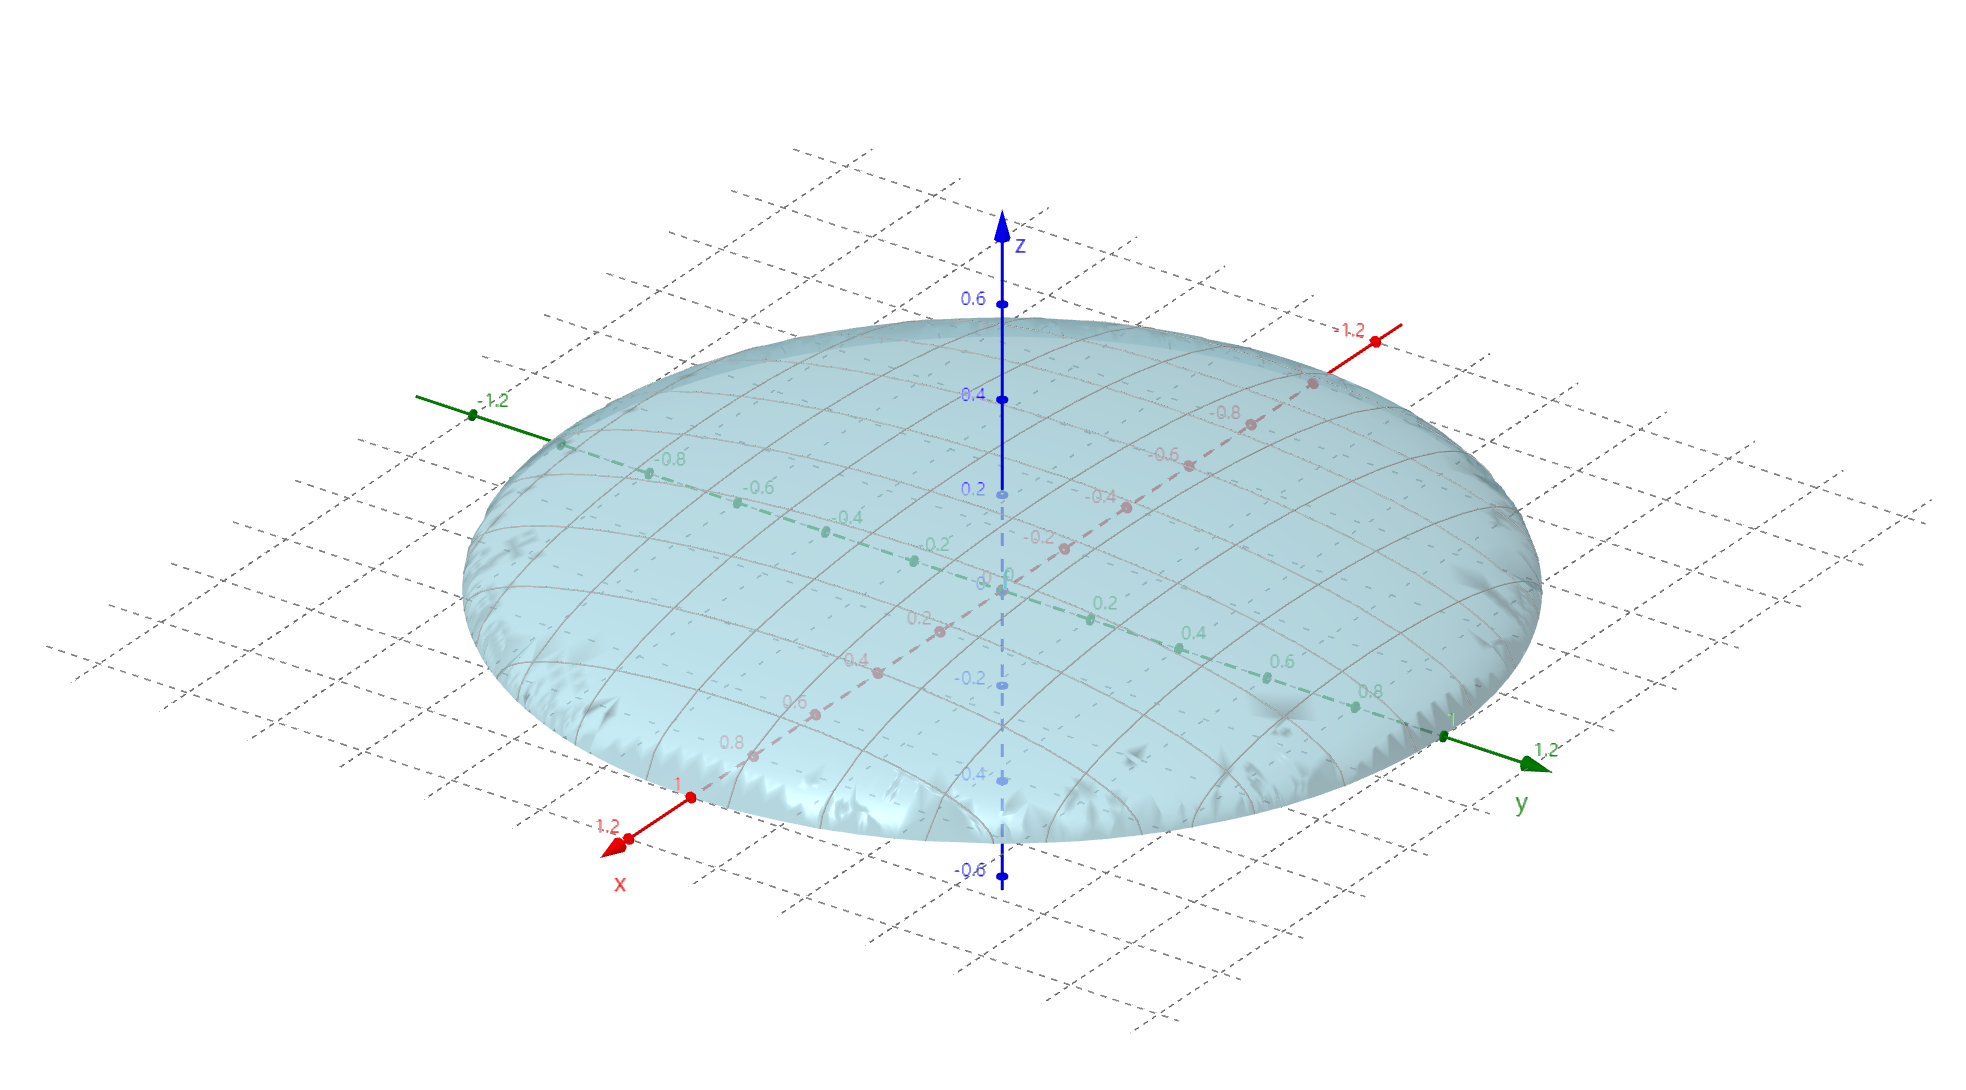
\includegraphics[width = \textwidth]{3D-plot.png}
\end{center}

\subsubsection*{c.}

\begin{align*}
	P\{X^2 + Y^2 \leq \frac{1}{2}\} &= \iint_{x^2 + y^2 \leq \frac{1}{2}} f(x,y) \mathrm{d}x \mathrm{d}y \\
	&= \iint_{x^2 + y^2 \leq \frac{1}{2}} \frac{3}{2\pi} \sqrt{1 - x^2 - y^2} \mathrm{d}x \mathrm{d}y \\
	&= \frac{3}{2\pi} \int_{0}^{2\pi} \int_{0}^{\frac{1}{\sqrt{2}}} \sqrt{1 - r^2} r \mathrm{d}r \mathrm{d}\theta \\
	&= \frac{3}{2\pi} \int_{0}^{2\pi} \left[-\frac{1}{3} (1 - r^2)^{\frac{3}{2}}\right]_{0}^{\frac{1}{\sqrt{2}}} \mathrm{d}\theta \\
	&= \frac{3}{2\pi} \int_{0}^{2\pi} \frac{1}{3} - \frac{1}{3} \cdot \frac{1}{2\sqrt{2}} \mathrm{d}\theta \\
	&= \frac{2\sqrt{2} - 1}{2\sqrt{2}}
\end{align*}

\subsubsection*{d.}

\begin{align*}
	f_X(x) &= \int_{-\sqrt{1-x^2}}^{\sqrt{1-x^2}} \frac{3}{2\pi} \sqrt{1 - x^2 - y^2} \mathrm{d}y \\
	&= \frac{3}{2\pi} \int_{-\sqrt{1-x^2}}^{\sqrt{1-x^2}} \sqrt{1 - x^2 - y^2} \mathrm{d}y \\
	&= \frac{3}{4} (1 - x^2)
\end{align*}
同理可得$f_Y(y) = \frac{3}{4} (1 - y^2)$。

\begin{equation*}
	f_X(x) =
	\begin{cases}
		\frac{3}{4} (1 - x^2), & -1 \leq x \leq 1 \\
		0, & \text{otherwise}
	\end{cases}
\end{equation*}
\begin{equation*}
	f_Y(y) =
	\begin{cases}
		\frac{3}{4} (1 - y^2), & -1 \leq y \leq 1 \\
		0, & \text{otherwise}
	\end{cases}
\end{equation*}

\subsubsection*{e.}

\begin{align*}
	f_{X|Y}(x|y) &= \frac{f(x,y)}{f_Y(y)} \\
	&= \frac{\frac{3}{2\pi} \sqrt{1 - x^2 - y^2}}{\frac{3}{4} (1 - y^2)} \\
	&= \frac{2\sqrt{1 - x^2 - y^2}}{\pi(1 - y^2)} \\
	f_{Y|X}(y|x) &= \frac{f(x,y)}{f_X(x)} \\
	&= \frac{\frac{3}{2\pi} \sqrt{1 - x^2 - y^2}}{\frac{3}{4} (1 - x^2)} \\
	&= \frac{2\sqrt{1 - x^2 - y^2}}{\pi(1 - x^2)}
\end{align*}

\subsection*{补充1}

\subsubsection*{(1)}

已知$f_{Y|X}(y|x) = \frac{1}{x}$,则$X$与$Y$的联合分布函数为:
\begin{align*}
	f_{X,Y}(x,y) &= f_{Y|X}(y|x) f_X(x) \\
	&= \frac{1}{x} \cdot 1 \\
	&= \frac{1}{x}
\end{align*}
\begin{equation*}
	f_{X,Y}(x,y) =
	\begin{cases}
		\frac{1}{x}, & 0 < y < x < 1 \\
		0, & \text{otherwise}
	\end{cases}
\end{equation*}

\subsubsection*{(2)}

\begin{align*}
	f_Y(y) &= \int_y^1 f(x,y) \mathrm{d}x \\
	&= \int_y^1 \frac{1}{x} \mathrm{d}x \\
	&= \ln x \bigg|_y^1 \\
	&= -\ln y
\end{align*}

\subsubsection*{(3)}

\begin{align*}
	P\{X + Y > 1\} &= P\{Y > 1 - X\} \\
	&= \int_{\frac{1}{2}}^1 \int_{1-x}^x f(x,y) \mathrm{d}y \mathrm{d}x \\
	&= \int_{\frac{1}{2}}^1 \int_{1-x}^x \frac{1}{x} \mathrm{d}y \mathrm{d}x \\
	&= \int_{\frac{1}{2}}^1 \frac{1}{x} \left[y\right]_{1-x}^x \mathrm{d}x \\
	&= \int_{\frac{1}{2}}^1 \frac{1}{x} (x - 1 + x) \mathrm{d}x \\
	&= \int_{\frac{1}{2}}^1 2 - \frac{1}{x} \mathrm{d}x \\
	&= \left[2x - \ln x\right]_{\frac{1}{2}}^1 \\
	&= 1 - \ln 2
\end{align*}

\subsection*{补充2}

\subsubsection*{(1)}

边缘密度函数为:
\begin{align*}
	f_X(x) &= \int_x^{\infty} e^{-y} \mathrm{d}y \\
	&= -e^{-y} \bigg|_x^{\infty} \\
	&= e^{-x} \\
	f_Y(y) &= \int_0^y e^{-y} \mathrm{d}x \\
	&= ye^{-y}
\end{align*}
\begin{equation*}
	f_X(x) =
	\begin{cases}
		e^{-x}, & x > 0 \\
		0, & \text{otherwise}
	\end{cases}
\end{equation*}
\begin{equation*}
	f_Y(y) =
	\begin{cases}
		ye^{-y}, & y > 0 \\
		0, & \text{otherwise}
	\end{cases}
\end{equation*}

易知$X$和$Y$不独立,因为$f(x,y) = e^{-y} \neq f_X(x)f_Y(y) = ye^{-x}e^{-y}$。

\subsubsection*{(2)}

\begin{align*}
	f_{X|Y}(x|y) &= \frac{f(x,y)}{f_Y(y)} \\
	&= \frac{e^{-y}}{ye^{-y}} \\
	&= \frac{1}{y} \\
	f_{Y|X}(y|x) &= \frac{f(x,y)}{f_X(x)} \\
	&= \frac{e^{-y}}{e^{-x}} \\
	&= e^{x-y}
\end{align*}
\end{document}